% =============================================================
%  DLBDSOOFPP01 — Habit Tracking App
%  Portfolio Part 1: Conception Phase
%  Author: Alejandro Diaz Roque  |  MatrNo: <YOUR MATRICULATION NUMBER>
%  Date:   <YYYY-MM-DD>
%
%  Compile with:  pdflatex conception.tex
%  Output:        conception.pdf
%
%  Target length: 1–3 DIN A4 pages (as per assignment brief).
%
%  NOTE ON DIAGRAMS:
%    Both diagrams are drawn directly in LaTeX using TikZ,
%    so no external image files (uml.png / flow.png) are needed.
%    Compile twice so TikZ references resolve correctly.
% =============================================================

\documentclass[11pt,a4paper]{article}

% ---------- Encoding & fonts ----------
\usepackage[utf8]{inputenc}
\usepackage[T1]{fontenc}
\usepackage{lmodern}
\usepackage{microtype}

% ---------- Language ----------
\usepackage[english]{babel}

% ---------- Page geometry (DIN A4, 2 cm margins) ----------
\usepackage[a4paper,margin=2cm]{geometry}

% ---------- Line spacing 1.5 ----------
\usepackage{setspace}
\onehalfspacing

% ---------- Graphics & diagrams ----------
\usepackage{graphicx}
\usepackage{float}
\usepackage{caption}
\captionsetup{font=small,labelfont=bf}

% ---------- TikZ for native diagrams ----------
\usepackage{tikz}
\usetikzlibrary{
  shapes.geometric,
  arrows.meta,
  positioning,
  fit,
  backgrounds,
  calc
}

% ---------- Tables ----------
\usepackage{booktabs}
\usepackage{tabularx}
\usepackage{array}

% ---------- Lists ----------
\usepackage{enumitem}
\setlist{itemsep=2pt,topsep=4pt}

% ---------- Hyperlinks ----------
\usepackage[hidelinks]{hyperref}

% ---------- Code listings ----------
\usepackage{listings}
\usepackage{xcolor}
\lstset{
  basicstyle=\ttfamily\small,
  keywordstyle=\color{blue!70!black},
  commentstyle=\color{gray},
  stringstyle=\color{green!50!black},
  breaklines=true,
  frame=single,
  rulecolor=\color{gray!40},
  showstringspaces=false,
  columns=fullflexible,
}

% ---------- Header / footer ----------
\usepackage{fancyhdr}
\pagestyle{fancy}
\fancyhf{}
\fancyhead[L]{\small DLBDSOOFPP01 — Portfolio Part 1}
\fancyhead[R]{\small Alejandro Diaz Roque}
\fancyfoot[C]{\thepage}
\renewcommand{\headrulewidth}{0.4pt}

% =============================================================
\begin{document}

% ---------- Title block ----------
\begin{center}
  {\LARGE\bfseries Habit Tracking App — Conception Phase}\\[4pt]
  {\large Portfolio Part 1 — Written Concept}\\[10pt]
  \begin{tabular}{rl}
    \textbf{Author:}       & Alejandro Diaz Roque \\
    \textbf{Matr.\ No.:}   & <YOUR MATRICULATION NUMBER> \\
    \textbf{Course:}       & DLBDSOOFPP01 — Object-Oriented and Functional Programming with Python \\
    \textbf{Date:}         & \today \\
    \textbf{Repository:}   & \href{https://github.com/<user>/<repo>}{github.com/<user>/<repo>} \\
  \end{tabular}
\end{center}

\vspace{6pt}
\hrule
\vspace{12pt}

% =============================================================
\section{Introduction and Motivation}
% =============================================================

\noindent


The client requires a Python backend for a habit tracking application that is
scheduled to be rolled out later this year. The task focuses on the essential
functionality of such an application — defining habits, checking them off, and
analysing progress over time — without providing any graphical user interface.
The design must combine \textbf{object-oriented programming} for the habit
domain and \textbf{functional programming} for the analytics layer, and it
must expose this logic through a clean, usable interface.


% =============================================================
\section{Problem Definition and Scope}
% =============================================================

\noindent


\subsection*{In scope}
\begin{itemize}
  \item Habit definition with a name, description, and periodicity
        (at least \emph{daily} and \emph{weekly}).
  \item Checking off a habit task at any point in time.
  \item Persistence of habits and their completions between sessions.
  \item Analytics over the stored data (list habits, filter by periodicity,
        longest streak overall and per habit).
  \item A command line interface (CLI) for user interaction.
  \item A REST API exposing the same core logic over HTTP (FastAPI).
  \item A unit test suite covering the critical components.
\end{itemize}

\subsection*{Out of scope}
\begin{itemize}
  \item Any graphical user interface or mobile client.
  \item Authentication and multi-user support.
  \item Notifications, reminders, or cloud synchronisation.
  \item Use or modification of existing third-party habit trackers.
\end{itemize}

% =============================================================
\section{Concept and Core Idea}
% =============================================================

\noindent


\medskip
\noindent
\textbf{Core idea.} 

\medskip
\noindent
\textbf{Why a layered architecture?} 

% =============================================================
\section{Proposed Solution and Architecture}
% =============================================================

\noindent


\subsection{Domain Model (Object-Oriented)}

The central abstraction is the \texttt{Habit} class. Each habit carries a
\texttt{name}, a \texttt{description}, a \texttt{periodicity}
(\texttt{"daily"} or \texttt{"weekly"}), a \texttt{created\_at} timestamp,
and a collection of \texttt{Completion} objects. A \texttt{HabitTracker}
orchestrates creation, deletion, check-off, and retrieval of habits. A
\texttt{Storage} component encapsulates persistence, and an
\texttt{Analytics} module provides read-only, functional access to the data.

\medskip
\noindent


\subsection{Analytics Layer (Functional Programming)}

The analytics module is deliberately implemented in the functional paradigm.
Every analytics function is \emph{pure}: it takes the tracker (or a list of
habits) as input and returns a new value without mutating its arguments.
Streak computation is expressed as a \texttt{functools.reduce} over a sorted,
deduplicated sequence of completion dates (or ISO weeks for weekly habits).

\medskip
\noindent


\subsection{Persistence}

Habit data is stored in a \textbf{SQLite} database accessed through Python's
built-in \texttt{sqlite3} module. The schema consists of two tables,
\texttt{habits} and \texttt{completions}, linked by a foreign key with
\texttt{ON DELETE CASCADE}. This choice avoids external dependencies, supports
indices and constraints, and matches the brief's recommendation of a
database-backed solution over a plain file store.

\medskip
\noindent


\subsection{User Interaction: CLI and REST API}

Two thin adapters sit on top of the shared core:

\begin{itemize}
  \item A \textbf{CLI} built with \texttt{Typer}, offering commands such as
        \texttt{create}, \texttt{delete}, \texttt{check-off}, \texttt{list},
        and \texttt{analyse longest-streak}.
  \item A \textbf{REST API} built with \texttt{FastAPI}, exposing the same
        operations over HTTP with automatic OpenAPI documentation at
        \texttt{/docs}.
\end{itemize}

Neither adapter contains business logic; both delegate to
\texttt{HabitTracker} and \texttt{Analytics}.

\medskip
\noindent


% =============================================================
\section{Architecture Diagrams}
% =============================================================

\noindent


% -------------------------------------------------------------
% Figure 1 — UML class diagram (drawn natively in TikZ)
% -------------------------------------------------------------
\begin{figure}[H]
  \centering
  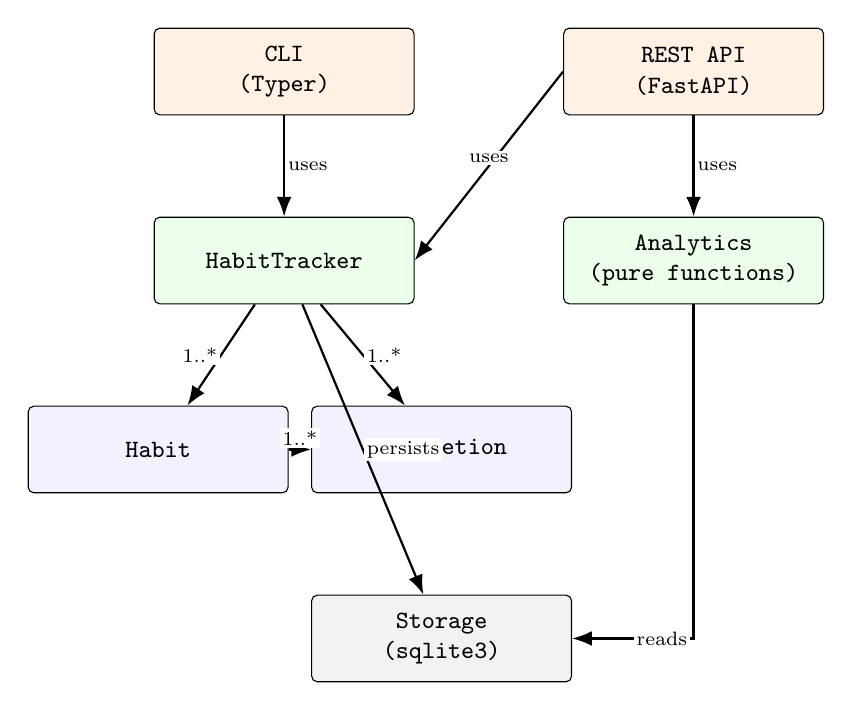
\begin{tikzpicture}[
      class/.style={
        draw,
        rectangle,
        rounded corners=2pt,
        minimum width=3.3cm,
        minimum height=1.1cm,
        align=center,
        font=\small\ttfamily,
        fill=blue!5
      },
      adapter/.style={
        draw,
        rectangle,
        rounded corners=2pt,
        minimum width=3.3cm,
        minimum height=1.1cm,
        align=center,
        font=\small\ttfamily,
        fill=orange!10
      },
      core/.style={
        draw,
        rectangle,
        rounded corners=2pt,
        minimum width=3.3cm,
        minimum height=1.1cm,
        align=center,
        font=\small\ttfamily,
        fill=green!8
      },
      storage/.style={
        draw,
        rectangle,
        rounded corners=2pt,
        minimum width=3.3cm,
        minimum height=1.1cm,
        align=center,
        font=\small\ttfamily,
        fill=gray!10
      },
      rel/.style={-{Latex[length=2.5mm]}, thick},
      lbl/.style={font=\scriptsize, midway, fill=white, inner sep=1pt}
    ]

    % --- Layer 1: adapters ---
    \node[adapter] (cli) at (0,0)    {CLI\\(Typer)};
    \node[adapter] (api) at (5.2,0)  {REST API\\(FastAPI)};

    % --- Layer 2: core ---
    \node[core]  (tracker)   at (0,-2.4)   {HabitTracker};
    \node[core]  (analytics) at (5.2,-2.4) {Analytics\\(pure functions)};

    % --- Layer 3: domain ---
    \node[class] (habit)      at (-1.6,-4.8) {Habit};
    \node[class] (completion) at (2.0,-4.8)  {Completion};

    % --- Layer 4: storage ---
    \node[storage] (storage) at (2.0,-7.2) {Storage\\(sqlite3)};

    % --- Relations ---
    \draw[rel] (cli) -- (tracker)      node[lbl,right]{uses};
    \draw[rel] (api) -- (analytics)    node[lbl,right]{uses};
    \draw[rel] (api.west) -- (tracker.east) node[lbl,above]{uses};

    \draw[rel] (tracker) -- (habit)      node[lbl,left]{1..*};
    \draw[rel] (tracker) -- (completion) node[lbl,right]{1..*};
    \draw[rel] (habit)   -- (completion) node[lbl,above]{1..*};

    \draw[rel] (tracker) -- (storage) node[lbl,right]{persists};
    \draw[rel] (analytics.south) |- (storage.east)
        node[lbl,pos=0.75,right]{reads};

  \end{tikzpicture}

  \caption{UML class diagram of the habit tracking application. The green
  nodes form the framework-agnostic core; orange nodes are thin adapters
  (CLI, REST API); grey is the persistence layer.}
  \label{fig:uml}
\end{figure}

% -------------------------------------------------------------
% Figure 2 — Interaction / flow diagram (drawn natively in TikZ)
% -------------------------------------------------------------
\begin{figure}[H]
  \centering
  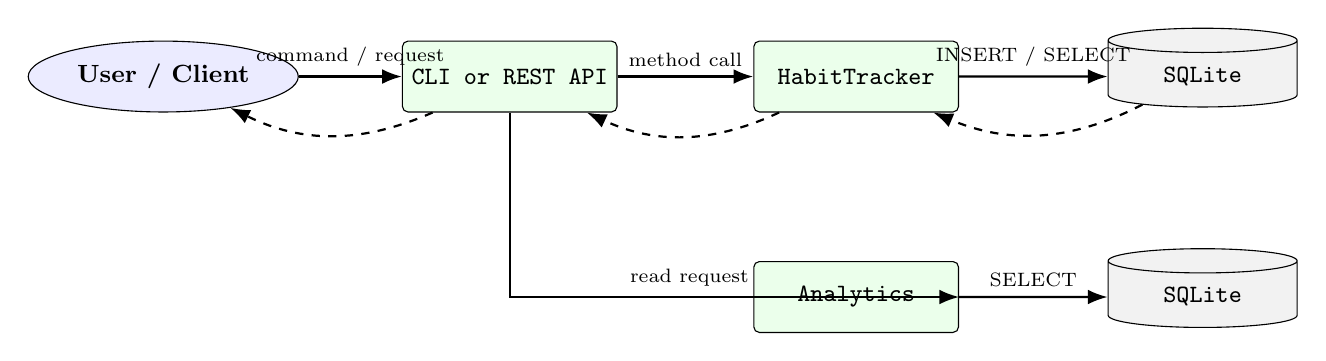
\begin{tikzpicture}[
      node distance=1.4cm and 1.6cm,
      actor/.style={
        draw, ellipse, minimum width=2.2cm, minimum height=0.9cm,
        align=center, font=\small\bfseries, fill=blue!8
      },
      comp/.style={
        draw, rectangle, rounded corners=2pt,
        minimum width=2.6cm, minimum height=0.9cm,
        align=center, font=\small\ttfamily, fill=green!8
      },
      store/.style={
        draw, cylinder, shape border rotate=90, aspect=0.25,
        minimum width=2.4cm, minimum height=1.0cm,
        align=center, font=\small\ttfamily, fill=gray!10
      },
      ar/.style={-{Latex[length=2.5mm]}, thick},
      albl/.style={font=\scriptsize, above, midway}
    ]

    % --- Write path (top row) ---
    \node[actor] (user)   at (0,0)    {User / Client};
    \node[comp]  (iface)  at (4.4,0)  {CLI or REST API};
    \node[comp]  (trk)    at (8.8,0)  {HabitTracker};
    \node[store] (db)     at (13.2,0) {SQLite};

    \draw[ar] (user)  -- (iface) node[albl]{command / request};
    \draw[ar] (iface) -- (trk)   node[albl]{method call};
    \draw[ar] (trk)   -- (db)    node[albl]{INSERT / SELECT};

    % --- Read path (bottom row) ---
    \node[comp]  (ana) at (8.8,-2.8) {Analytics};
    \node[store] (db2) at (13.2,-2.8) {SQLite};

    \draw[ar] (iface.south) |- (ana.east)
        node[albl,pos=0.7]{read request};
    \draw[ar] (ana) -- (db2) node[albl]{SELECT};

    % --- Return arrows ---
    \draw[ar, dashed] (db)  to[bend left=25]  (trk);
    \draw[ar, dashed] (trk) to[bend left=25]  (iface);
    \draw[ar, dashed] (iface) to[bend left=25] (user);

  \end{tikzpicture}

  \caption{Interaction flow. Top row: write path
  (\texttt{User} $\rightarrow$ \texttt{CLI/API} $\rightarrow$
  \texttt{HabitTracker} $\rightarrow$ \texttt{SQLite}). Bottom row: read
  path for analytics. Both adapters delegate to the same core.}
  \label{fig:flow}
\end{figure}

% =============================================================
\section{Methodology and Tooling}
% =============================================================

\noindent


\begin{table}[H]
  \centering
  \small
  \begin{tabularx}{\textwidth}{@{}l l X@{}}
    \toprule
    \textbf{Concern} & \textbf{Tool / Choice} & \textbf{Justification} \\
    \midrule
    Language        & Python $\geq$ 3.11   & Modern typing, required by the brief ($\geq$ 3.7). \\
    Domain model    & OOP (\texttt{dataclasses}/classes) & Encodes the habit concept explicitly. \\
    Analytics       & Functional paradigm (\texttt{map}, \texttt{filter}, \texttt{reduce}) & Required by the brief for analytics. \\
    Persistence     & \texttt{sqlite3} (stdlib) & No external deps, real schema, recommended by brief. \\
    CLI             & \texttt{Typer}       & Declarative, testable, auto-help. \\
    REST API        & \texttt{FastAPI} + \texttt{uvicorn} & Automatic OpenAPI docs, Pydantic validation. \\
    Testing         & \texttt{pytest}, \texttt{pytest-cov}, \texttt{httpx} & Mature ecosystem, coverage reporting. \\
    \bottomrule
  \end{tabularx}
  \caption{Overview of chosen tools and the reasoning behind each choice.}
  \label{tab:tools}
\end{table}

\medskip
\noindent


% =============================================================
\section{Plan of Procedure}
% =============================================================

\noindent


\begin{enumerate}
  \item \textbf{Phase 1 — Conception (this document).} Define scope, domain
        model, analytics design, persistence, and interfaces; produce the UML
        and flow diagrams.
  \item \textbf{Phase 2 — Development / Reflection.} Implement the core
        (\texttt{Habit}, \texttt{HabitTracker}, \texttt{Storage},
        \texttt{Analytics}), then the two adapters (CLI, FastAPI), followed by
        the fixture data and the unit test suite.
  \item \textbf{Phase 3 — Finalization.} Refine the implementation after tutor
        feedback, finalise the README and API documentation, publish the
        repository on GitHub, and submit the abstract PDF together with a ZIP
        of all three phases.
\end{enumerate}

\medskip
\noindent


% =============================================================
\section{Testing Strategy}
% =============================================================

\noindent


The critical parts of the solution — the validity of the habit tracking
components and the analytics module — are covered by a \texttt{pytest} suite.
Tests target:

\begin{itemize}
  \item \textbf{Models and tracker:} creation, validation errors, check-off,
        deletion, retrieval, cascade removal of completions.
  \item \textbf{Analytics:} empty history, single completion, consecutive
        streaks, broken streaks, weekly ISO-week handling, periodicity
        filtering.
  \item \textbf{Storage:} schema initialisation, round-trip save/load,
        parameterised queries, foreign-key cascade.
  \item \textbf{Adapters:} CLI smoke tests via \texttt{CliRunner}; REST API
        tests via \texttt{TestClient} covering 201/204/404/422 responses.
\end{itemize}

\medskip
\noindent


% =============================================================
\section{Expected Outcome and Success Criteria}
% =============================================================

\noindent


The finished product is a Python package that:

\begin{itemize}
  \item lets users create, delete, and check off daily and weekly habits;
  \item persists all state in a local SQLite database;
  \item ships with five predefined habits and four weeks of example tracking
        data as a reproducible test fixture;
  \item provides functional analytics: list all habits, list by periodicity,
        longest streak overall, longest streak per habit;
  \item exposes the same logic through both a CLI and a documented REST API;
  \item includes a passing unit test suite runnable with a single
        \texttt{pytest} command;
  \item is documented with a README and Python docstrings, and is hosted on a
        public GitHub repository.
\end{itemize}

\medskip
\noindent


% =============================================================
\section{Conclusion}
% =============================================================

\noindent


The conception phase establishes a clear separation between the
framework-agnostic domain core and the two user-facing adapters, aligns each
part of the system with the paradigm mandated by the brief (OOP for habits,
functional for analytics), and lays out a concrete, testable path from
concept to finished product.

\medskip
\noindent


% =============================================================
% References (optional — uncomment if you cite anything)
% =============================================================
% \section*{References}
% \addcontentsline{toc}{section}{References}
% \begin{thebibliography}{9}
%   \bibitem{assignment}
%     Internationale Hochschule (IU).
%     \textit{DLBDSOOFPP01 — Assignments Portfolio}.
%     Course material, <YEAR>.
% \end{thebibliography}

\end{document}